\documentclass[11.5pt]{article}

%BEGIN_FOLD Packages

%\documentclass{sig-alternate}
\usepackage{multicol}
\usepackage[utf8]{inputenc}
\usepackage{color}
%\usepackage{lipsum}
\usepackage{xcolor}
\usepackage[colorlinks,linkcolor=navy,citecolor=blue]{hyperref}
%\usepackage{verbatim}
%\usepackage{textcomp}
%\usepackage{tabularx}
%\usepackage{csquotes}
\usepackage{comment}
\usepackage{array}
\usepackage{geometry}
\usepackage{amsmath}
\usepackage[toc,page]{appendix}
%\usepackage[english]{babel}
\usepackage{graphicx}
\usepackage{mathtools}  
\usepackage{environ}  
\usepackage{ulem}
\usepackage{tikz}
\usetikzlibrary{arrows}
\usepackage{pgfplots}
\usepackage{pdfpages}
\usepackage{nicefrac} % in package 'units'
\usepackage{twoopt}
\usepackage{makecell}
\usepgfplotslibrary{fillbetween}
\usetikzlibrary{patterns}
\usepackage{courier}
\usepackage{forloop}% http://ctan.org/pkg/forloop
%\usepackage{physics}
\usepackage{changepage}
%\usepackage[labelsep=endash]{caption}
\usepackage{caption}


%END_FOLD
%BEGIN_FOLD Definitions


\NewEnviron{eq}{
	\begin{align} % \begin{equation}\begin{split}
	\BODY
	\end{align} % \end{split}\end{equation}
}

\mathtoolsset{showonlyrefs}


%\usepackage[document]{ragged2e} % imports the package ragged2e and left-justifies the text
%\raggedright 

\newcolumntype{L}[1]{>{\raggedright\let\newline\\\arraybackslash\hspace{0pt}}m{#1}}
\newcolumntype{C}[1]{>{\centering\let\newline\\\arraybackslash\hspace{0pt}}m{#1}}
\newcolumntype{R}[1]{>{\raggedleft\let\newline\\\arraybackslash\hspace{0pt}}m{#1}}


\definecolor{navy}{HTML}{000080} 

\geometry{
	letterpaper,
	left=20mm,
	right=20mm,
	top=23mm,
	bottom=27mm,
}

\setlength\columnsep{20pt}


\renewenvironment{abstract}
{\small
	\begin{center}
		\bfseries Remarks \vspace{-.5em}\vspace{0pt}
	\end{center}
	\list{}{%
		\setlength{\leftmargin}{50mm}% <---------- CHANGE HERE
		\setlength{\rightmargin}{\leftmargin}%
	}%
	\item\relax}
{\endlist}

\newenvironment{colfigure} {
		\par\medskip\noindent\minipage{\linewidth}
	} {
		\endminipage\par\medskip
	}

%\newenvironment{coltable}[2][h]{
%	\begin{center}
%		\begin{tabular}[#1]{#2}
%	} { 
%		\end{tabular}
%%		\captionof{table}{#1}
%%		\label{table:missing}
%	\end{center}
%	}


\pgfplotsset{
	discard if/.style 2 args={
		x filter/.code={
			\edef\tempa{\thisrow{#1}}
			\edef\tempb{#2}
			\ifx\tempa\tempb
			\def\pgfmathresult{inf}
			\fi
		}
	},
	discard if not/.style 2 args={
		x filter/.code={
			\edef\tempa{\thisrow{#1}}
			\edef\tempb{#2}
			\ifx\tempa\tempb
			\else
			\def\pgfmathresult{inf}
			\fi
		}
	}
}





%END_FOLD
%BEGIN_FOLD Commands




\renewcommand{\L}{\left(}
\newcommand{\R}{\right)}
\newcommand{\noi}{\noindent}
\newcommand{\thetaB}{\boldsymbol{\theta}}
\newcommand{\curvyL}{\mathcal{L}}
\newcommand{\lra}{\Leftrightarrow}
\newcommand{\uda}{\Updownarrow}
\newcommand{\ti}[1] {\textit{#1}}
\newcommand{\fn}[1] {\footnote{#1}}
\newcommand{\m}[1]{ \begin{bmatrix} #1 \end{bmatrix} }
\renewcommand{\det}[1]{ \begin{vmatrix} #1 \end{vmatrix} }
\renewcommand{\b}[1]{ \boldsymbol{#1} }
\newcommand{\tb}[1] {\textbf{#1}}
\renewcommand{\bf}[1]{ \textbf{#1} }
\newcommand{\eqs}{ \begin{align} }
\newcommand{\eqe}{ \end{align} }
%\newcommand{\be}[1]{ \begin{#1} }
%\newcommand{\l}{\left(}
\renewcommand{\thesubsection}{\thesection.\alph{subsection}}  % use letters for subsections
\newcommand{\subsectionnote}[2]{ \subsection[#1]{#1\footnote{#2} } }
\newcommand{\wB}[0]{ \b{w} }
\newcommand{\xB}[0]{ \b{x} }
%\def\x \b{x}
\newcommand\gauss[2]{1/(#2*sqrt(2*pi))*exp(-((x-#1)^2)/(2*#2^2))} 
\newcommand\nGauss{\mathcal{N}}
\renewcommand{\t}[1]{  \text{#1}  }
\newcommand{\gaussFunctionText}[3]{ % 1=param/x, 2=mean/mu, 3=variance/sigma
	\frac{1}{ (#3)  \sqrt{2\pi}}  \exp \( - \frac {(#1- #2 )^2}{(2)  (#3) ^2}  \)
}
\newcommand{\hlineB}{  \Xhline{4\arrayrulewidth}   }  

\newcommand\plotfill[3]{
	\path[name path=#1Ground] (axis cs:#2,0) -- (axis cs:#3,0);  % just a horisontal line on the x-axis?
	\addplot [
	thick,
	color=blue,
	fill=blue, 
	fill opacity=0.1
	] 
	fill between[
	of=#1 and #1Ground,
	soft clip={domain=#2:#3},
	];	
}
\newcommand\ifrac[2]{\nicefrac{#1}{#2}}
\newcommand\half{{\nicefrac{1}{2}}}

\newcommand\tc[1]{\texttt{#1}}
\newcommand\calc[1]{   \pgfmathparse{#1}\pgfmathresult    }

\newcommand{\classificationError}[1]{ 
  1 - max #1
}
%\newcommand{\classification}[1]{ 
%	-	\sum_{k}^{k_{#1}}  {f_k}_{#1}\log_2 {f_k}_{#1} 
%}


\newcounter{myLoopCounter}
\newcommand{\repeatValue}[2][1]{%
	\forloop{myLoopCounter}{0}{\value{myLoopCounter}<#1}{#2}%
}

\newcommand{\note}[1]{   \parbox{15em}{#1}   }

	
%\def\norm#1{\left\|#1\right\|}
%\let\xB\b{x}
%\let\svvert\abe
%\let\Skod\left(

%\let\svverta\L(
%\let\svvertb\R)

\def\paranthesize#1{}

\def\i#1/#2{ \ifrac{#1}{#2}  }
\def\(#1\){\left(#1\right)}

\def\[#1\]{\left[#1\right]}

%\def\#1\\#2{\left[#1\right]}


%\def \'#1){\b{#1}}

\def\~#1{{ \widetilde{#1} }}


%\def\!#1\!{  \pgfmathparse{#1}\pgfmathresult  }


\pgfmathdeclarefunction{gauss}{2}{ 
	% #1=mean (mu), #2=variance (sigma)
	\pgfmathparse{1/(#2*sqrt(2*pi))*exp(-((x-#1)^2)/(2*#2^2))}%
}


%END_FOLD

%%%%%%%%%%%%%%%%%%%%%%%%%%%%%%%%%%%

%\usepackage[dvipsnames]{xcolor}
%\usepackage[dvipsnames]{xcolor}
%
%\usepackage{fancyvrb}
%
%% redefine \VerbatimInput
%\RecustomVerbatimCommand{\VerbatimInput}{VerbatimInput}%
%{fontsize=\footnotesize,
%	%
%	frame=lines,  % top and bottom rule only
%	framesep=2em, % tion between frame and text
%%	rulecolor=\color{Gray},
%	%
%%	label=\fbox{\color{Black}data.txt},
%	label=\fbox{data.txt},
%	labelposition=topline,
%	%
%	commandchars=\|\(\), % escape character and argument delimiters for
%	% commands within the verbatim
%	commentchar=*        % comment character
%}
%

%%%%%%%%%%%%%%%%%%%%


\def\datapath{../data}

\begin{document}



%BEGIN_FOLD Frontpage
	

\title{
	Predicting survival rates of the Titanic \\using machine learning techniques\\ (the Kaggle dataset) }
%	\numberofauthors{1} 
\author{
	Rune Munkholm Jensen\\
}
\date{}

\maketitle

%\section{Abbreviations}
%\lipsum[2]


%END_FOLD		
			
\newpage
%			
%\flushbottom
%\raggedbottom			

\twocolumn
%\begin{multicols}{2}			
			

\newcommand{\dataFigure}[3][width=0.75\linewidth]{
	\begin{colfigure}
		\centering
		\includegraphics[#1]{\datapath/image/#2}
\captionof{figure}{\small #3}
		\label{fig:#2}
	\end{colfigure}
}			
\newcommand{\fullWidthDataFigure}[3][width=0.75\linewidth]{
	\begin{figure*}
		\centering
		\includegraphics[#1]{\datapath/image/#2}
		\captionof{figure}{\small #3}
		\label{fig:#2}
	\end{figure*}
}			

%\newcommand{\myTable}[2]{
%	\begin{center}
%		\begin{tabular}#2\end{tabular}
%		\captionof{table}{#1}
%%		\label{table:missing}
%	\end{center}	
%	}			




%\newcommand{\coltable}[3][!ht]{
%\begin{center}
%	\begin{tabular}[#1]{#2}
%	%	\caption{Missing entries count in the training data set.}
%	\captionof{table}{Missing entries count in the training data set. Three attributes has missing values.}
%	\label{table:missing}
%\end{center}
%}			
%


			
\section{Strategy}
The strategy taken will be to identify good data for generalization, by visualizing the correlation between attributes and survival. A starting point is to identify those  attributes  that appear to generalize well in terms of predicting survival directly, i.e. where the value range of the attribute has a clear and obvious correlation with survival outcome. 

Once relevant attributes have been identified, these will be prepared for machine learning algorithms by predicting (filling in) missing values, a step generally necessary since most machine learning algorithms do not work well (or at all) with missing data. The methods chosen for modeling missing values for different attributes may differ, depending on the assumed nature of the data specific to each particular attribute.

Next, we will use the training data and an appropriate machine learning algorithm to produce a model for predicting survival and finally evaluate the model's accuracy on the test data set to see how well we fared. The results may come in handy the next time one is to escape a sinking early nineteen-hundreds steamship in icy waters, although they do unfortunately come a bit too late for the good folks aboard the \ti{Titanic}. We will proceed anyway, however, in the name of science.

\section{Missing data}
An overview of  missing data for the train and test sets is given by  tables \ref{table:missing} and \ref{table:missingTest}.


\begin{center}
	\begin{tabular}[!ht]{|c|c|} \hline
		Attribute & Count \\  \hlineB
		Age & 177 \\ \hline 
		Cabin & 687 \\ \hline 
		Embarked & 2 \\ \hline 
		Fare & 0 \\ \hline 
		Name & 0 \\ \hline 
		Parch & 0 \\ \hline 
		Pclass & 0 \\ \hline 
		Sex & 0 \\ \hline 
		SibSp & 0 \\ \hline 
		Survived & 0 \\ \hline 
		Ticket & 0 \\ \hline 
	\end{tabular}
%	\caption{Missing entries count in the training data set.}
	\captionof{table}{Missing entries count in the training data set. Three attributes have missing values: \ti{Age}, \ti{Cabin} and \ti{Embarked}	.}
	\label{table:missing}
\end{center}


\begin{center}
	\begin{tabular}[!ht]{|c|c|} \hline
		Attribute & Count \\  \hlineB
		Age & 86 \\ \hline 
		Cabin & 327 \\ \hline 
		Embarked & 0 \\ \hline 
		Fare & 1 \\ \hline 
		Name & 0 \\ \hline 
		Parch & 0 \\ \hline 
		Pclass & 0 \\ \hline 
		Sex & 0 \\ \hline 
		SibSp & 0 \\ \hline 
		Survived & (hidden by Kaggle) \\ \hline 
		Ticket & 0 \\ \hline 
	\end{tabular}
	%	\caption{Missing entries count in the training data set.}
	\captionof{table}{Missing entries count in the test data set. Three attributes have missing values: \ti{Age}, \ti{Cabin} and \ti{Fare}. }
	\label{table:missingTest}
\end{center}


\section{Relevant attributes}

Here, the attributes that are identified as relevant to survival are outlined.

\subsection*{Gender}
Interestingly, it appears from the attribute \ti{Sex}, shown in figure \ref{fig:sex-survival2}, that females had a slightly better chance of survival. This could possibly indicate that emotional nature/response to the impact was beneficial in abandoning the ship in time. 
%On speculate that the majority of the staff were reluctant to leave their role and that these have likely been men, given that there were twice as many men as women onboard. 
	

%\dataFigure{sex-survival}{Females appear to slightly better chances of survival, as is seen by the higher mortality rate of men.}

\dataFigure{sex-survival2}{Females (right) fared far better in the crucial moments, compared to men (left).}

\subsection*{Age}

Age also appears to be a key factor, as seen in figure \ref{fig:age-survival}. Clearly, young infants may have benefited from adult and female  supervision, but then mortality takes dominance abruptly from working age and remains high thereafter.

% (presumably a result of the substantial amount of crew\fn{$\i{\#crew}/{\#passengers} = \i1324/{2223}\approx 60\% $, derived from \text{http://www.titanicfacts.net/titanic-passengers.html} }) 

\dataFigure{age-survival}{Age versus survival, with opposing trends at each end of the spectrum.}

%\begin{figure*}
%	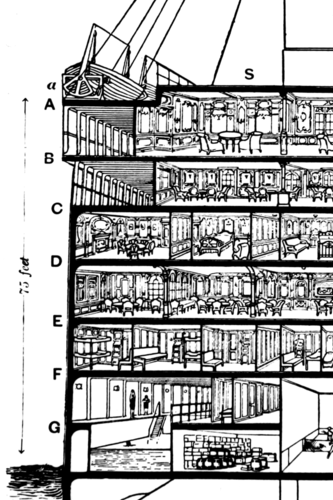
\includegraphics[width=\textwidth]{../data/image/decks}
%	\caption{This is a tiger.}
%\end{figure*}


\subsection*{Fare}

Also seen is that \ti{Fare} has a strong influence on survival, as shown in figure \ref{fig:fare-survival}.

\dataFigure[width=0.9\linewidth]{fare-survival}{More money, more survival.}


\subsection*{Social class}

Somewhat related to \ti{Fare} is the social class, as indicated by the \ti{Pclass} attribute. As one might expect, figure \ref{fig:pclass-survival}  similarly shows that the higher the class, the better the chance of survival.

\dataFigure{pclass-survival}{Survival for social classes 1 through 3, left to right. By far most of the people on the lowest of the classes perished. }


\section{Irrelevant attributes}

Some attributes are presumed to be irrelevant by nature for generalizing on the target label, \ti{Survival}. These will therefore be discarded: \ti{PassengerId} (a linearly increasing number),  \ti{Name} (presumed to be random characters) and \ti{Ticket} (a string generated independently from any other data). 

In addition, attributes that have not been chosen as relevant in the previous will discarded too, due to either being assumed irrelevant, noisy or highly correlated with another relevant attribute. 

For an example of the latter, we note that embarkation location also have  something to say about survival, as shown in figure \ref{fig:embark-survival}, with slightly diminished survival for those that embarked at Southampton.

\dataFigure[width=0.5\linewidth]{embark-survival}{Embarkation and survival, with Southampton on the far right.}

However, we note that this is highly similar to the previous figure \ref{fig:pclass-survival} for social class, indicating that embarkation is highly correlated social class. Comparing the two, as shown in figure  \ref{fig:embarked-pclass}, we get the intuitive overview: most of the lower class boarded at Southampton, an early 1900s industrial city, and these were also the ones that got the short end of the stick in terms of survival. 

\dataFigure[width=0.5\linewidth]{embarked-pclass}{Embarkation versus social class, with Southampton on the far right and lowest class on top.}



\section{Additional attributes}

To play around with potential hidden information, some assumptions will be made that allows for extracting additional attributes, as described in the following. 

\subsection*{Name length}

We will assume that, in general, fancy people of the early 1900s fancied to carry fancy names and that simple people would be given simple names. For instance, a  low-status blacksmith would have been named "John Blacksmith", as opposed to "Distinguished Service Order and Military Pink Cross recipient by the Queen and Emir of Arabia, Sir Lord John Smithsonian Grandius of All Blacksmiths and Foreign Subjectables". 

With this assumption in mind, we may introduce an additional attribute, \ti{NameLength}, that will hopefully  provide some indication of class. The assumption made here, is that people of class are more likely to mingle with other people of class, but may carry a ticket that reflects this to a lesser extent (the other way around would be unfathomable, as fancy folks will always try and suck up to those upwards in the hirearchy of fanciness, not downwards). Hence, people with long names may, in general, have been higher above the waterline, because the fancy folks wanted to be on top - and thus  may have had better chances of survival. 

As the derived figure \ref{fig:nameLength} shows, this correlation does in fact exist and that long names are well worth the effort it in the long run. 

%Also, and not surprisingly, people carrying a ticket of higher class are also somewhat more likely to have longer names, as shown in figure \ref{fig:nameLength}, although what we are trying to capture here are extra notions of class that may not be directly encoded in the original registration of class. 

\dataFigure{nameLength}{People with short names (small x-values) appear to have had the odds against them in terms of survival.}

%\dataFigure[width=0.6\linewidth]{nameLengthVsClass}{Name length versus class 1 through 3. The names of low-class people are clustered in the 12-30 interval, whereas high-class names are more spread out.}



% \ref{fig:decks}.

%\dataFigure[width=0.2\linewidth]{deck-survival}{Survival by deck.}

\subsection*{Cabin deck and number}

The \ti{Cabin} attribute is given to us as zero-to-many string tokens, each composed of both the deck letter and cabin number, which is difficult to generalize on. We may instead parse this as two respective attributes, settling on the first string token as the primary  (to guard against  cases where multiple tokens are given). 


\dataFigure[width=0.5\linewidth]{decks}{The decks of the Titanic, each indentified by the letters A through G (a T deck also exists in the training data, which was the boat deck on the very top).}


\def\fnDeckPlans{
\fn{Using the deck plans available on \url{www.encyclopedia-titanica.org/titanic-deckplans/}}
}



The intuition behind how we may use this information, is clear from  the prior knowledge we have on how the ship sunk: the crew were  sailing above the speed limit in the Atlantic and struck an ice berg almost head-on, after which the ship began to pivot around the gravitational center of  its longitudinal axis, slowly emerging the cabins from the bow and lower decks\fn{Anyone that saw the  blockbuster movie \ti{Titanic} will be able to confirm that this is in fact how things went down} (had the crew instead been trying to parallel park their way to New York, then we would  have expected the ship to have sunk from the rear). We thus have  the misère\fn{French for "misery"} shown in figure \ref{fig:sinking}, from which one could  guess that passengers at higher deck levels and higher cabin numbers had better chances of survival\fnDeckPlans.




\dataFigure[width=0.5 \linewidth]{sinking}{An artist's captivating dramatization of the gradual sinking, which is currently serving as cute child coloring material on \url{onlycoloringpages.com}. For passengers genuinely interested in maintaining good health, cabins at the stern (rear) are obviously preferable at this point in time and may thus, to the statistician that came after, be an indicator of post-disaster longevity. }

As seen in figure \ref{fig:deck-survival2}, survival does differ between the decks (making it a useful attribute) and surprisingly decks D and E appear to have been optimal. 

\dataFigure[width=0.9 \linewidth]{deck-survival2}{From left to right, survival for decks A through T. Here, fancy folks on the top deck did not have the upper hand in terms of survival.}

Also, we see from figure \ref{fig:cabin-survival} that higher cabin numbers do not necessarily imply higher survival, as one could initially assume due to decreasing proximity to the (increasing) waterline. However, there does appear to a noticeable optimum in terms of survival, around cabin numbers 30, making the cabin number an informative attribute.

\dataFigure{cabin-survival}{Survival for increasing cabin numbers.}



\section{Data prep, missing values}
 
% As previously shown, \ti{Gender} has proven to be an 
 
 
 \subsection*{Missing values for age}

When comparing age to survival, as shown in figure \ref{fig:age}, it could appear that age roughly follows a Gaussian distribution that differs slightly between survivors and non-survivors. This simplification obviously does not capture all intricacies perfectly, most notable the sudden drop around adolescence/adult age and the increasing spike towards infancy. One could certainly easily explain the latter quirks by speculating that adolescents were kept in school up up until a specific age regardless of class - and perhaps affirmative action was showing its filthy face when filling up the life boats, i.e. favoring women and children.

\dataFigure{age}{$Age$ could appear to follow a Gaussian distribution.}


\dataFigure[width=0.6\linewidth]{modelAgeDead}{Fitting a Gaussian to age on men (assumed to be non-survivors).}
\dataFigure[width=0.6\linewidth]{modelAgeSurvived}{Fitting a Gaussian to age on females (assumed to be survivors).}

To deal with these peculiarities we will assume this: the age distribution on board the Titanic followed a Gaussian, but infants introduced an additional Gaussian of their own, making it a multimodal distribution. To simplify a bit, we will model these two distributions individually: we ignore the affect of the over-representation of infants on the general age and model the infants separately using some age threshold. When sampling, we will then randomly choose to sample from  the infant distribution at the same fraction as the infant group composes of the entire group (infants + non-infants). 

Furthermore, we will separate the cases for survivors and non-survivors, since they appear to differ somewhat. But since we do not have the prediction label \ti{Survived} available for the test set, we will rely on the strong correlation between survival and gender: females will be assumed to be survivors  in general and men non-survivors. This fitting is shown in detail in \ref{fig:modelAgeDead} and \ref{fig:modelAgeSurvived}. 

In numbers, the infant thresholds (as chosen by visual inspection) are $Age < 11$ for females and $age <14$ for men, yielding the 'infant' models shown in figures \ref{fig:modelAgeSurvivedUnder11} and \ref{fig:modelAgeDeadUnder14}. 	



% abrupt cutoff, we will, for each survival outcome, discard any randomly sampled \ti{age} value that falls below these thresholds in favor of yet another sample, taken from the Gaussian  formed from age 0 and up to the threshold. More precisely, these thresholds, determined by visual inspection, are $Age < 11$ for $Survived = 1$ and $age <14$ for  $Survived = 0$, as shown in figures \ref{fig:modelAgeSurvivedUnder11} and \ref{fig:modelAgeDeadUnder14}. 

\dataFigure[width=0.6\linewidth]{modelAgeSurvivedUnder11}{Fitting a Gaussian to females (survivors) under age 11.}
\dataFigure[width=0.6\linewidth]{modelAgeDeadUnder14}{Fitting a Gaussian to men (non-survivors) under age 14.}

Clearly, survival predictions appear to become more fluctuant at these lower intervals, but we will justify the choice of model by the assumption that the probabilities of finding any children aboard drops sharply at both ends of the 'infant' intervals, and hence, the Gaussian will certainly be superior to e.g.  simply taking mean values. 

We could also have chosen to refine the fraction of infant samples by investigating which distribution has the highest likelihood. Technically, this would have been done by finding the fraction of infants up until the age at which the two Gaussians intersect, although this could seem less correct given the abrupt (not smooth) cutoff for adults. This idea is exemplified in figure \ref{figure:gaussianIntersect} using the survival attribute from the train set.

	\begin{center}
		\begin{tikzpicture}
		\begin{axis}[ 
		xlabel={Age},			
		ytick=\empty,
%		axis lines=left, 
%		xtick=\empty, ytick=\empty
		ylabel={},
				domain=0:80,						
		y label style={
			rotate=-90,
		},
	%				xmin=0, 
	%				xmax=10, 				
		]
		\addplot[
			scatter,
			only marks,
			color=red,
			mark size=0.3mm,
	%		point meta=explicit symbolic,
			scatter/classes={
				Age={color=red,line width=0mm}
		%		P={mark=*,mark size=4pt,green,draw=black},%
		%		n={mark=*,mark size=2pt,red!30!white,draw=black},%
		%		N={mark=*,mark size=4pt,red,draw=black}%
				%		a={mark=*,mark size=4pt,green!70!black,draw=black,pin=135:{\color{black}$(65, 35)$},label={(65, 35)}] {}
			},
			discard if not={Survived}{0}
			] 	
			table[meta=Survived,col sep = tab] {\datapath/age(sorted,unique).csv};
%		\addplot[mark=none, smooth, color=red!30!white,line width=0.5mm] { (0.0683962264151) * \gauss{6.0}{3.55567956133} + (1-0.0683962264151)  * \gauss{30.6261792453}{14.1721098771}};			
%		\addplot[mark=none, smooth, color=red!60!white,line width=0.2mm] { (1-0.0683962264151)  * \gauss{30.6261792453}{14.1721098771}};			
%		\addplot[mark=none, smooth, color=red!60!white,line width=0.2mm] { (0.0683962264151) * \gauss{6.0}{3.55567956133}};			
		\addplot[mark=none, smooth, color=red!60!white,line width=0.4mm] {  \gauss{30.6261792453}{14.1721098771}};			
		\addplot[mark=none, smooth, color=red!60!white,line width=0.4mm] {  \gauss{6.0}{3.55567956133}};			
		\end{axis}
		\end{tikzpicture}
			\captionof{figure}{Age for non-survivors modeled by two guassians that have (positive) intersect at $Age= 13.3339$. The right Gaussian is modeled for all non-survivors, and the left for all survivors under age 14.}
			\label{figure:gaussianIntersect}			
	\end{center}

 \subsection*{Missing values for deck(number)}

Reinvestigating the previously shown figure \ref{fig:deck-survival2}, it could appear that deck allocations follow a Gaussian distribution that would be almost identical for each survival outcome (hence, we will not branch on survival assumptions for this attribute). A single Gaussian model, as shown in figure \ref{fig:modelDeck},   will therefore be used to model missing values for decks.

\dataFigure[width=0.6\linewidth]{modelDeck}{Fitting a Gaussian to deck numbers for all passengers.}


\subsection*{Missing values for deck cabin}

As previously shown in figure \ref{fig:cabin-survival}, there is a tendency for increased survival for a subrange of the cabin numbers, although survival is generally very intermingled for this attribute, as shown in figure \ref{fig:deckCabin-survival}.

\dataFigure[width=0.9\linewidth]{deckCabin-survival}{Deducing survival trends based on cabin numbers is messy business.}

 To complicate things further, the allocation of cabin numbers do not follow the longitudinal axis of the ship in a strict sense and the individual decks vary wildly in layout, with some having sections dedicated to various types of common or functional areas. Figures \ref{fig:modelDeckACabinDead} through \ref{fig:modelDeckGCabinSurvivors} shows attempts at cracking this by binning up and fitting a Gaussian to each deck (again branching on gender as a pseudo-survival indicator).

\begin{center}
%	\captionof{table}{Survival for all decks.}
	\begin{tabular}[!ht]{C{0.22\linewidth}C{0.22\linewidth}} 
		\dataFigure[width=1\linewidth]{modelDeckACabinDead}{Deck A.}
		 & \dataFigure[width=1\linewidth]{modelDeckACabinSurvivors}{Deck A} \\
		\dataFigure[width=1\linewidth]{modelDeckBCabinDead}{Deck B.}
		& \dataFigure[width=1\linewidth]{modelDeckBCabinSurvivors}{Deck B} \\
		\dataFigure[width=1\linewidth]{modelDeckCCabinDead}{Deck C.}
		& \dataFigure[width=1\linewidth]{modelDeckCCabinSurvivors}{Deck C} \\
		\dataFigure[width=1\linewidth]{modelDeckDCabinDead}{Deck D.}
		& \dataFigure[width=1\linewidth]{modelDeckDCabinSurvivors}{Deck D} \\
		\dataFigure[width=1\linewidth]{modelDeckECabinDead}{Deck E.}
		& \dataFigure[width=1\linewidth]{modelDeckECabinSurvivors}{Deck E} \\	
		\dataFigure[width=1\linewidth]{modelDeckFCabinDead}{Deck F.}
		& \dataFigure[width=1\linewidth]{modelDeckFCabinSurvivors}{Deck F} \\
		\dataFigure[width=1\linewidth]{modelDeckGCabinDead}{Deck G.}
		& \dataFigure[width=1\linewidth]{modelDeckGCabinSurvivors}{Deck G} \\
	\end{tabular}
		\label{table:deckCabins}		
	%	\caption{Missing entries count in the training data set.}
\end{center}

However, the best, although not perfect, generalization appears when all decks are combined, as shown in figures \ref{fig:modelDeckCabinDeadPreCorrect} and  \ref{fig:modelDeckCabinSurvivorsPreCorrect}. 


\dataFigure[width=0.6\linewidth]{modelDeckCabinDeadPreCorrect}{Binning and fitting a Gaussian for man (all decks).}
\dataFigure[width=0.6\linewidth]{modelDeckCabinSurvivorsPreCorrect}{Binning and fitting a Gaussian for females (all decks).}


From these we get some resemblance of a bell curve, although the peak could appear to be skewed towards the lower cabin numbers, i.e. the bow (front) of ship. We will explain and accommodate this by assuming that the impact was felt and heard most violently at the general area of impact, the bow, provoking most fear amongst these passengers and higher tendency to flee, compared to those at the stern. A better fitted Gaussian may therefore arise by visually determining some mean and assuming an "imaginary" extension of the bow and passengers, with the left side of the mean symmetric to the right half  (of which we have data). Assuming visually estimated means and reflecting the data (as the "left half" of a bell curve), we get the resulting Gaussian fittings shown in figures \ref{fig:modelDeckCabinDead} and  \ref{fig:modelDeckCabinSurvivors}, both of which appear to capture the nature of the data better.

\dataFigure[width=0.6\linewidth]{modelDeckCabinDead}{Binning and fitting a Gaussian on men for all decks, assuming a mean of 30.}
\dataFigure[width=0.6\linewidth]{modelDeckCabinSurvivors}{Binning and fitting a Gaussian on females for all decks, assuming a mean of 27.}

Our model for filling in missing deck cabin numbers is therefore obtained by sampling positive values from one of these two models, as dictated by gender.



%
%When inspecting the deck plans for the lower decks, a reasonable explanation appears: as figure \ref{fig:deckE} reveals, these cabins are located between two of the ships main staircases, both of which are not spaced far apart. 
%
%\fullWidthDataFigure[width=0.8 \linewidth]{deckE}{The ship had two closely located staircases around cabin numbers 25-40, here shown for the E deck.}




%\dataFigure[width=0.9\linewidth]{modelDeckCabin}{Fitting a Gaussian to deck 		cabin numbers for all passengers.}

%\begin{center}
%	\begin{tikzpicture}
%	\begin{axis}[
%	every axis plot post/.append style={
%		mark=none,
%		domain=1.5:5,
%		samples=50,
%		smooth
%	}, % All plots: from -2:2, 50 samples, smooth, no marks
%	axis x line=bottom, % no box around the plot, only x and y axis
%	axis y line=left, % the * suppresses the arrow tips
%	enlargelimits=upper,
%	line width=0.25mm,
%	xlabel={$gpa$},			
%	ylabel={$\nGauss (gpa \mid \mu, \sigma^2)$},			
%	y label style=
%	{
%		at={(ticklabel* cs:1.05)},
%		rotate=-90,
%		%			anchor=west,
%	},		
%	] % extend the axes a bit to the right and top
%	\addplot {\gauss{3.4}{0.42}};
%	%%		\addlegendentry{label=H}
%	\addplot {\gauss{3}{0.2433}};
%	%		\addlegendentry{label=N}
%	\node [above] at (axis cs:  4, 1.3) {\tiny $p(GPA \mid Label = N)$};
%	\node [above] at (axis cs: 4.65, 0.5) {\tiny $p(GPA \mid Label = H)$};
%	\end{axis}
%	\end{tikzpicture}
%\end{center}


%\dataFigure[width=0.7\linewidth]{age-age}{A small drop in passengers appear}

\subsection*{Missing values for fare}

A single fare value is missing in the test data. Under the assumption that a single observation has little impact, it will simple be filled in by the mean of the fares in the set.


%\subsection*{bla bla}

%Figure xxx shows this, following the normalization of attributes, to avoid attributes in greater numeric ranges dominating those in smaller numeric ranges (as well as avoid large numerical values in potential future dots products).
%
%

%
%
%Figure xxx shows this, following the normalization of attributes, to avoid attributes in greater numeric ranges dominating those in smaller numeric ranges (as well as avoid large numerical values in potential future dots products).
%

\section{Implementation}

\subsection*{Technology Choices}

The model was implemented in Python using \ti{Numpy} and \ti{Panda}. A conversion from Panda frames to the Weka ARFF format allowed for using Weka's excellent inspection tools, to get an overview of the data. 

For training and classification,  a random forest was used from the \ti{scikit-learn} library since, although rendering our search for missing values less relevant, they are fast and was assumed to be of low risk to the desire for undertaking computational heavy parameter sweep and cross-fold validation operations. Furthermore, they are robust to outliers, of which no action was taken to guard against here. In addition, it was assumed that the  several hundred observations we have for each  data set is adequate for the 'randomization' to take affect. 

\subsection*{Optimizing accuracy}

An optimal \ti{n\_estimators} parameter value (the number of trees in the forest)  was determined by sweeping through the range 1-300 and picking the parameter that gave the greatest accuracy. For each sweep, accuracy was determined using the mean average precision of a ten-fold cross-validation: the training set was divided into blocks of ten, each tested by a model obtained from training on the remaning 9 blocks (hence, 10 rounds in total, each yielding $\i1/{10}$ contribution to the final accuracy of the sweep). 


\section{Results}

\subsection*{Train accuracy}

For the parameter sweeping of the training set, an optimal \ti{n\_estimators} parameter value of 25 was obtained along with mean average precisions,  as shown in figure \ref{fig:sweep}. It is seen that the solution found is most likely a fluctuation spike around a trend that could appear to still be rising with increasing parameter value. Hence, a slightly better parameter could perhaps be found by investigating minima over averaged data points.

	\begin{center}
		\begin{tikzpicture}
\begin{axis}[ 
		xlabel={n\_estimators},			
%		ytick=\empty,
		%		axis lines=left, 
		%		xtick=\empty, ytick=\empty
		ylabel={Accuracy},
%		domain=0:80,						
		y label style={
%			rotate=-90
		},
		%				xmin=0, 
		%				xmax=10, 				
		]
		\addplot[
			scatter,
%			only marks,
			color=red,
			mark size=0.3mm,
			%		point meta=explicit symbolic,
			scatter/classes={
				map={color=red,line width=0mm}
				%		P={mark=*,mark size=4pt,green,draw=black},%
				%		n={mark=*,mark size=2pt,red!30!white,draw=black},%
				%		N={mark=*,mark size=4pt,red,draw=black}%
				%		a={mark=*,mark size=4pt,green!70!black,draw=black,pin=135:{\color{black}$(65, 35)$},label={(65, 35)}] {}
			}
%			,discard if not={Survived}{0}
		] 	
		table[col sep = comma]{\datapath/predictionParamSweep.csv};
\end{axis}
\end{tikzpicture}
		\captionof{figure}{Parameter sweep accuracies.}
		\label{fig:sweep}			
	\end{center}




\subsection*{Test accuracy}

For the accuracy of the submission, the Kaggle leaderboard reports 0.75120 (username "RuneJensen"). It it seen that the test accuracy is slightly lower than the train cross-fold accuracy, which was anticipated given that the model was evaluated on unseen data that is likely to have slightly different variations of the general data patterns.





%	
%To get a sense of the data, we plot the correlation matrices for all combinationers, as seen in figure .....



%\begin{figure}[tph!]
%	\centerline{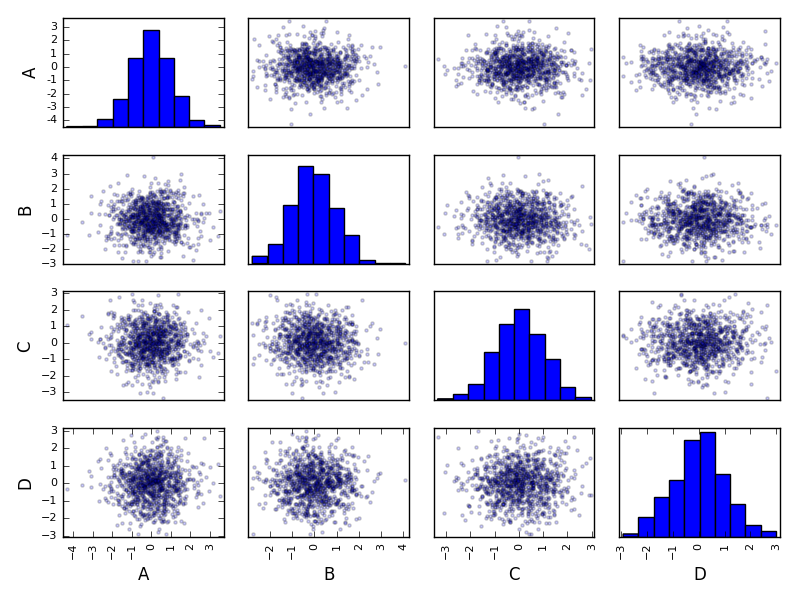
\includegraphics[totalheight=6cm]{../data/scatter_matrix.png}}
%	\caption{used by \citet[p.~4]{XXXXX}.}
%	\label{fig:verticalcell}
%\end{figure}


%\end{multicols}


\newpage

\begin{thebibliography}{9}
%	\bibitem{ngProg}
%	Arian Maleki and Tom Do, Review of Probability Theory (\url{http://cs229.stanford.edu/section/cs229-prob.pdf})
	\bibitem{Bishop}
	Christopher M. Bishop, Pattern Recognition and Machine Learning, 2006, ISBN-10: 0-387-31073-8	

	\bibitem{Nd}
	Andrew Ngs notes

	
%	\bibitem{WikiDecisionTree}
%	"Decision tree learning" on Wikipedia
%	
%	\bibitem{BackProp}
%	Backpropagation handout
%	
%	\bibitem{NN}
%	Michael Nielsen's ANN book, $http://neuralnetworksanddeeplearning.com/chap1.html$
	
	
%	\url{https://en.wikipedia.org/wiki/Decision_tree_learning}
\end{thebibliography}

%BEGIN_FOLD Appendices

\newpage


%END_FOLD

\end{document}
